\begin{figure}
\centering
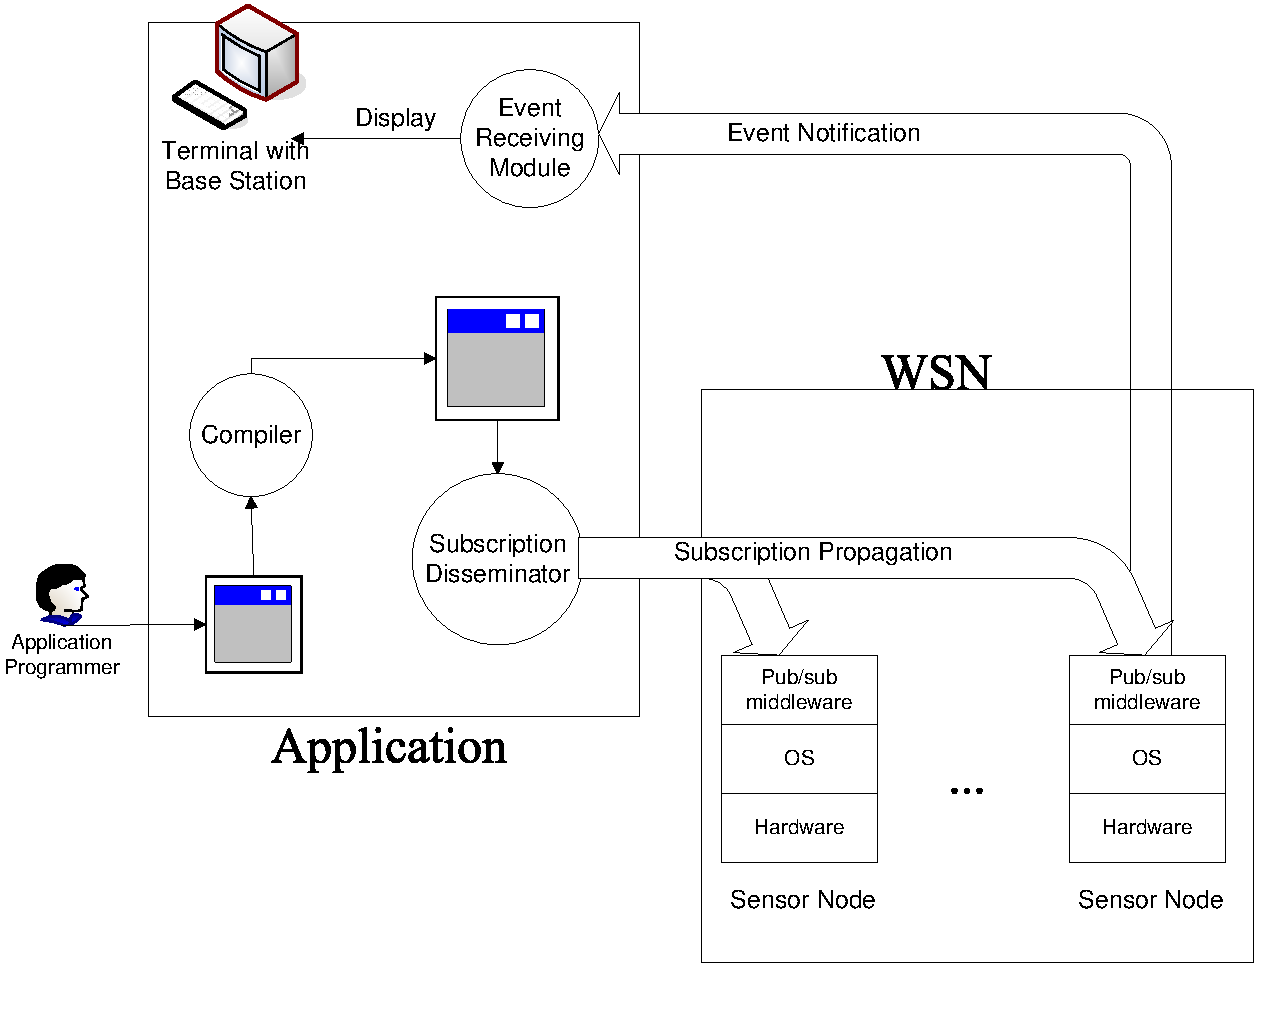
\includegraphics[width=.6\textwidth]{psware-architecture}
\caption{Event processing in PSWare}
\label{fig:psware-architecture}
\end{figure}

\section{Composite Event Processing in PSWare}
\label{sec:design}
In this section, we discuss how PSWare is designed to support composite event. The overall work flow of event processing in PSWare is shown in Figure \ref{fig:psware-architecture}. To use the middleware, applications developers will first define event types according to the application requirements. The subscription will then be compiled and processed by the EDL compiler and be disseminated into the network. When the events are detected by the sensor nodes, they will be delivered to the application.

\subsection{EDL Compiler}
\begin{figure}
\centering
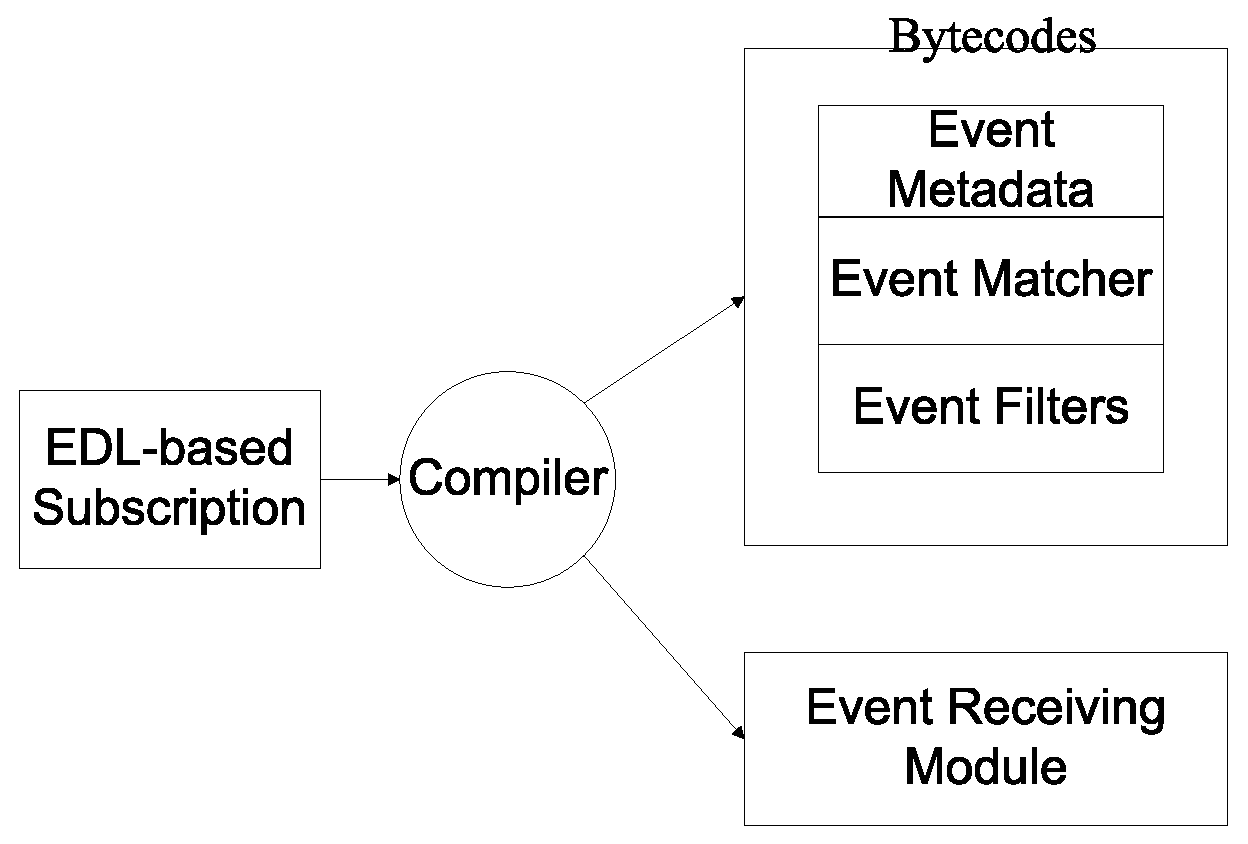
\includegraphics[width=.7\textwidth]{edlcompiler}
\caption{EDL compiler structure}
\label{fig:edlcompiler}
\end{figure}

Our Event Definition Language (EDL) is an implementation for our event-based programming model. For each EDL script, it contains one or more event definition and one subscribing statement. Formally, the BNF of the subscription is defined in Listing \ref{lst:BNFSubscription}.

\begin{lstlisting}[caption=BNF (simplified) of subscription, label=lst:BNFSubscription]
subscription -> event_declarations subscribe_statement
event_declarations -> event_declaration | event_declarations event_declaration
subscribe_statement -> SUBSCRIBE IDENTIFIER SEMICOLON
\end{lstlisting}

The subscribe statement simply uses the keyword 'subscribe' followed the event type name needed by the application. Each event type declaration can have up to three parts: the event body, the where clause and the on clause. The event body defines the attributes of the events. The on clause are used to specify the sub-events used by a composite event. The where clause defines the filter of the corresponding event type. Formally, the BNF of event type is defined in Listing \ref{lst:BNFEvent}

\begin{lstlisting}[caption=BNF (simplified) of event type, label=lst:BNFEvent]
event_declaration -> EVENT IDENTIFIER event_body on_clause_opt where_clause_opt
event_body -> { field_declarations_opt }
on_clause -> ON { subevent_declarations_opt }
where_clause -> WHERE { conditional_expression }
\end{lstlisting}

The on clause and the where clause are both optional in case if the event is primitive or does not have a filter. The on clause looks similar to the field declaration except sub-events instead of fields are declared. This is done for a clear code presentation and easier type checking. The where clause simply consists of conditional expressions so that the filters may be defined by specifying the operators.

\begin{comment}
A simple example of using EDL is shown in Listing \ref{lst:originaledl}. In this example, two events, 'SimpleEvent' and 'CompEvent' are defined. 'SimpleEvent' is a primitive event which occurs when the detected temperature reading is above certain threshold. 'CompEvent' is a composite event that is based on two events of 'SimpleEvent' and their time must satisfy a certain condition in order to indicate the occurrence of 'CompEvent'.
\begin{lstlisting}[caption=A simple EDL program, label=lst:originaledl]
Event SimpleEvent {
	int temp=System.temp;
	int id=System.id;
	int time=System.time;
} where {
	temp > 30
}
Event CompEvent {
} on {
	SimpleEvent e1 and
	SimpleEvent e2
} where {
	e2.time-e1.time=600
}
\end{lstlisting}
\end{comment}

The EDL-based subscription will be processed by our EDL compiler. The output of the compiler has two parts as shown in Figure \ref{fig:edlcompiler}. The first part is the byte codes which will be executed by individual sensors to detect events. The format and the organization of the byte codes are closely related to the event detection framework and customization of PSWare. We will go through these topics in the following sections.

\begin{figure}
\centering
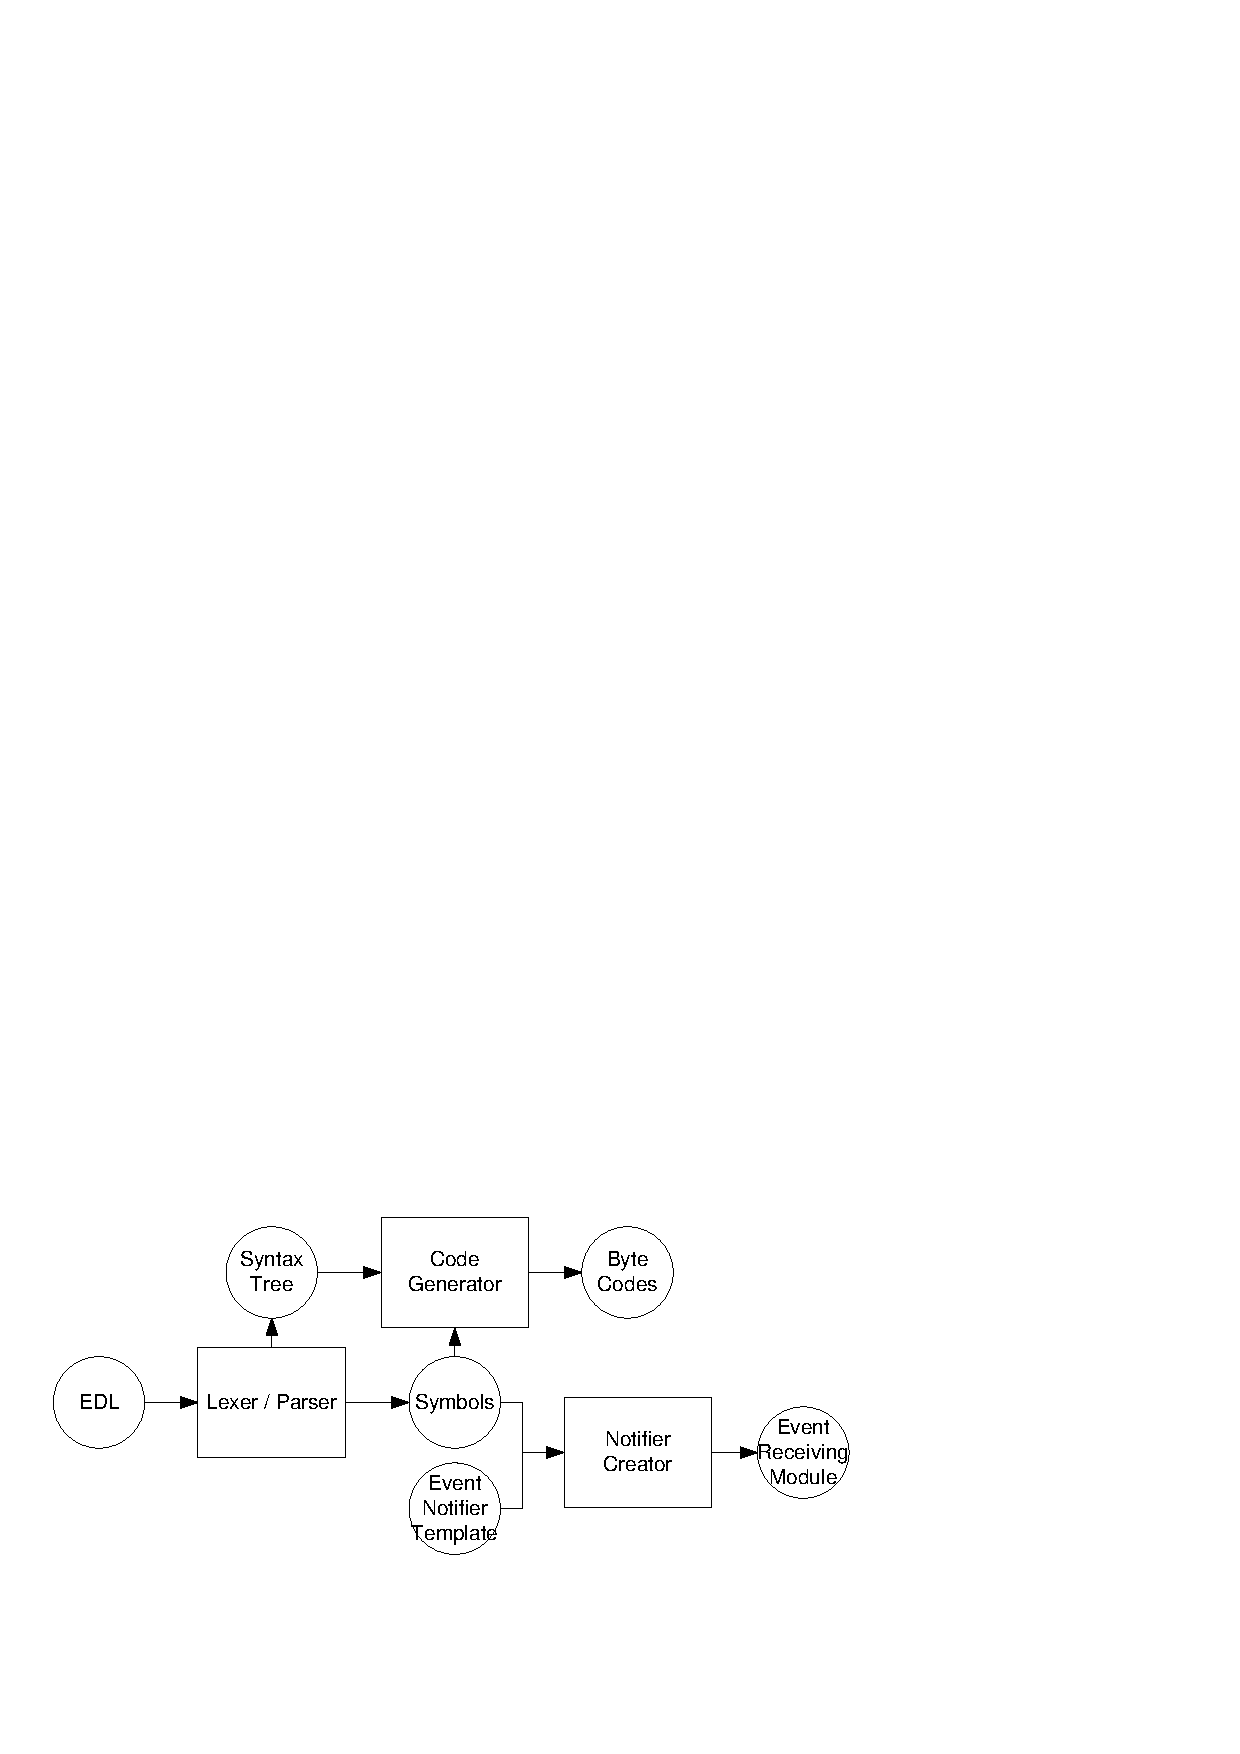
\includegraphics[width=.8\textwidth]{edlcompiler-flow}
\caption{EDL compiler flow}
\label{fig:edlcompiler-flow}
\end{figure}

The second part, the event receiving module is the implementation of the event notifier as discussed in Section \ref{sec:model}. As shown in Figure \ref{fig:edlcompiler-flow}, The EDL compiler will execute the following steps in order to generate the byte codes and event receiving module:
\begin{enumerate}
\item Parse the EDL script and generate the corresponding syntax tree and symbol table.
\item Generate the byte codes based on the syntax tree and symbol table.
\item Create the event receiving module based on the symbol table.
\end{enumerate}

\subsection{Event Detection Framework}
The byte codes generated by the compiler can be further divided into three parts: event meta data, event filters and event matcher. These components implements the programming interface discussed in Listing \ref{lst:pswareAPI} and \ref{lst:pswareEventMatcher}. Event meta data contains the description of the event types such as event type ID, event size and the individual attributes for each event. Event filters are the constraints defined for each event type. Event matcher schedules the execution for event detection according to the subscription and event relations.

The runtime environment on each sensor node is similar to the VM-based approach \cite{mate} in the sense that the subscriptions are broken down into some basic operations called instructions. Such design choice is for extensibility so that new features can be added more easily by adding new instructions. In addition to the VM-based runtime environment, each sensor node has an event buffer where the detected events can be stored for composite event detection.

\begin{figure}
\centering
\figurecurrentwidth{eventdetectionframework2}
\caption{Event detection framework}
\label{fig:eventdetectionframework2}
\end{figure}
The essential operations for our event detection framework is shown in Figure \ref{fig:eventdetectionframework2}. In this framework, the event matcher will first fetch the events from the event buffer and then evaluate them against the corresponding filters. If the event has been detected, then it will be transmitted over the network. Formally, the procedure of the event matcher can be shown in Procedure \ref{algo:eventmatcher} with some notations defined as:
\begin{itemize}
\item Event types: \(E=\{e_1, e_2 \cdots \}\)
\item For each \(e_n\in E\), its filter is: \(e_n\rightarrow filter\)
\item For each \(e_n\in E\), it has a set of events \(E_n=\{e_n^1, e_n^2 \cdots \}\) stored in the buffer.
\end{itemize}

\begin{algorithm}
\begin{algorithmic}
\REQUIRE \(E\)
	\FORALL {\(e_n\in E\)}
		\FORALL {\(e_n^i\in E_n\)}
			\IF {\(e_n\) is primitive}
				\STATE result = evaluate\_primitive (\(e_n^i\))
				\IF {result == True}
					\STATE eventMatched(\(e_n^i\))
					\IF {\(e_n\) is subscribed}
						\STATE deliver(\(e_n^i\))
					\ELSE
						\STATE forward(\(e_n^i\))
					\ENDIF
				\ENDIF
			\ELSE
				\STATE \(e_{sub} = \emptyset \)
				\FORALL {subevents \(e_m\) for \(e_n\)}
					\STATE \(e_{sub} = e_{sub}\bigcup selectSubevent (e_n, e_m)\)
				\ENDFOR
				\FORALL {subevents \(e_m\) for \(e_{sub}\)}
					\STATE evaluate\_composite(\(e_n^i\), \(e_m\), \(\cdots \))
				\ENDFOR
			\ENDIF
		\ENDFOR
	\ENDFOR
\end{algorithmic}
\caption{Procedure of the event matcher}
\label{algo:eventmatcher}
\end{algorithm}

There are several keys in the procedure. First, when the event matcher picks up the events of type \(e_n\) from the event buffer, it may use application specific mechanisms to pick up the desired events instead of trying all the possible combinations. Second, the 'deliver()' and the 'forward()' function are used to deliver the subscribed events or forward the events so that composite events may be detected. These two functions may also be application dependent to achieve high energy efficiency.

\begin{comment}
Figure \ref{fig:psware-interaction-simple} illustrates how different components in the middleware system interact with each other.

\begin{figure}
\centering
\figurecurrentwidth{psware-interaction-simple}
\caption{PSWare-E components interaction}
\label{fig:psware-interaction-simple}
\end{figure}
\subsection{PSWare Customization}
\end{comment}

Finally, it is necessary to mention the 'SystemEvent'. This module acts as the device driver for PSWare. It defines the sampling rate and a primitive event. All the fields of other events are obtained from 'System'. The module needs to implement three interfaces: StdControl, SystemClock and SystemEvent as shown in Listing \ref{lst:systemEvent}. StdControl is a module for initialization purpose. SystemClock defines the sampling frequency. SystemEvent is used to obtain the pointer to the 'System' event.

\begin{lstlisting}[caption=API of the 'System' event, label=lst:systemEvent]
module SystemEventM {
	provides {
		interface StdControl;
		interface SystemEvent;
		interface SystemClock;
	}
}
interface SystemEvent {
	command EventInstanceInfo * get();
}
\end{lstlisting}

The 'SystemEvent' is there so that needs to be implemented by the middleware developers as the  Once the 'System' event is defined, the application developers can further define their own functions for event delivery and event forwarding. We will show some examples in the next section. 